\begin{figure}[H]
    \centering
    \caption{Visualization of a 2-cube contained in $\Mult^{-1}(I) = (a,b)$}
    \label{Figure::helper_Mult_invers}
    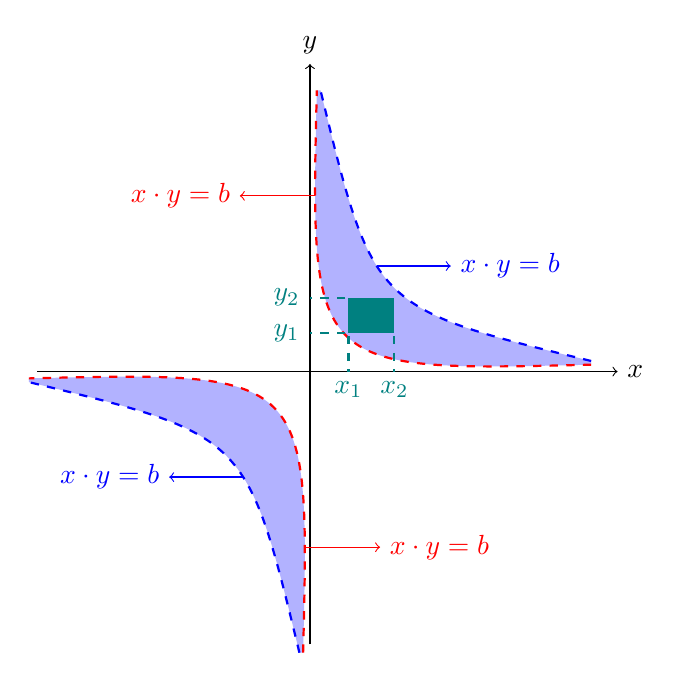
\begin{tikzpicture}[scale=0.67] % Scale everything to 2/3
    
        % Define parameters
        \def\a{1.33}  % Scaled to 2/3
        \def\b{3.33}  % Scaled to 2/3
        \def\xmin{-2.67}  % Scaled to 2/3
        \def\xmax{3.33}  % Scaled to 2/3
        \def\ymin{-2.67}  % Scaled to 2/3
        \def\ymax{3.33}  % Scaled to 2/3

        \fill[blue!30] 
        (\xmax+2, 0.13) .. controls (0,0) .. (0.13, \ymax+2)
        -- 
        (0.2, \ymax+2) .. controls (1.2,1.2) .. (\xmax+2, 0.2)
        -- cycle;

        % negative part
        \fill[blue!30] 
        (-0.13, -\xmax-2) .. controls (0,0) .. (-\ymax-2, -0.13)
        -- 
        (-\ymax-2, -0.2) .. controls (-1.2,-1.2) .. (-0.2, -\xmax-2)
        -- cycle;

        % positive part
        \draw[thick, red, dashed] (\xmax+2, 0.13) ..controls (0,0) .. (0.13, \ymax+2);
        \draw[thick, blue, dashed] (\xmax+2, 0.2) ..controls (1.2,1.2) .. (0.2, \ymax+2);
        
        % Reflected lines
        \draw[thick, red, dashed] (-0.13, -\xmax-2) .. controls (0,0) .. (-\ymax-2, -0.13);
        \draw[thick, blue, dashed] (-0.2, -\xmax-2) .. controls (-1.2,-1.2) .. (-\ymax-2, -0.2);

        % Axes
        \draw[->] (\xmin-2.5, 0) -- (\xmax+2.5, 0) node[right] {$x$};
        \draw[->] (0, \ymin-2.5) -- (0, \ymax+2.5) node[above] {$y$};

        % square
        \fill[teal] (0.73, 0.73) rectangle (1.6, 1.4);

        % labels
        \draw[thick, teal, dashed] (0.67,0.73) -- (0,0.73) node[left] {$y_1$};
        \draw[thick, teal, dashed] (1.6,0.67) -- (1.6,0) node[below] {$x_2$};
        \draw[thick, teal, dashed] (0.67,1.4) -- (0,1.4) node[left] {$y_2$};
        \draw[thick, teal, dashed] (0.73,0.67) -- (0.73,0) node[below] {$x_1$};

        % labels
        \draw[blue, ->] (1.27, 2) -- (2.67, 2) node[right] {$x \cdot y = b$};
        \draw[blue, ->] (-1.27, -2) -- (-2.67, -2) node[left] {$x \cdot y = b$};
        \draw[red, ->] (0.1, 3.33) -- (-1.33, 3.33) node[left] {$x \cdot y = b$};
        \draw[red, ->] (-0.1, -3.33) -- (1.33, -3.33) node[right] {$x \cdot y = b$};
        
    \end{tikzpicture}
\end{figure}
